\documentclass[10pt,a4paper]{article}
\usepackage[utf8]{inputenc}
\usepackage{amsmath}
\usepackage{amsfonts}
\usepackage{amssymb}
\usepackage{graphicx}
\usepackage{tikz}
\usetikzlibrary{positioning}

\DeclareMathOperator{\conv}{conv}

\newtheorem{observation}{Observation}

\begin{document}
	\section{Trivial example 1}
	Consider the graph
\begin{center}
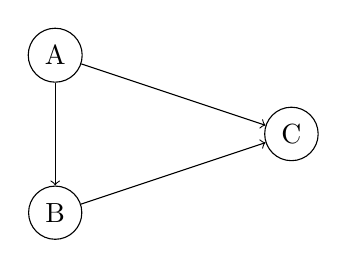
\begin{tikzpicture}
	\node[shape=circle,draw=black] (A) at (0,1) {A};
	\node[shape=circle,draw=black] (B) at (0,-1) {B};
	\node[shape=circle,draw=black] (C) at (3,0) {C};
	\draw[->] (A) edge (B);
	\draw[->] (A) edge (C);
	\draw[->] (B) edge (C);
	%\draw[color=gray] (0,0) -. (C);
\end{tikzpicture}
\end{center}
where $A$ is located at $(0,1)$, $B$ is located at $(0,-1)$ and $C$ is located at $(h,0)$. Denote the distance from $A$ or $B$ to $C$ by $l$. The supplies are $s_A = (1,0)$, $s_B = (0,1)$ and $s_C = (-1,-1)$. Consider the trivial cost function $c(x,y) = |x+y|$ where $x, y$ are the amounts of (signed) flow. Then
\[
\partial c(0,0) = \conv\left\{ (1,1),(-1,-1),(1,-1),(-1,1) \right\}
\]
or with inequalities $\partial c(0,0) = \{z:\, |e_i^T z| \leq 1 \,\forall i \}$. Obviously, an optimal flow is
\begin{align*}
f = \begin{pmatrix}
1&0\\0&1\\0&0
\end{pmatrix}.
\end{align*}
An optimal dual solution is $\phi_A = (l,l)$, $\phi_B = (l,l)$ and $\phi_C = (0,0)$. It can be easily checked that this satisfies all constraints. The derivative of $\phi$ is
\[
D\phi = \begin{pmatrix}
-l/h & 0\\-l/h & 0
\end{pmatrix}.
\]
We now check whether $D\phi$ meets the constraints, i.e. if $\lVert e_i^T D\phi \rVert\leq 1$. We see that $\lVert e_i^TD\phi \rVert = l/h > 1$ for all $i$. This is maybe surprising, as the flow $f$ is globally optimal (with respect to all possible graph topologies).
\begin{observation}
	Even if the global optimum is found, the dual constraints might not be satisfied.
\end{observation}
Since $e_i^T D\phi = (-l/h,0)$, this suggests that we should add an edge parallel to $(1,0)$ to the graph. We get:
\begin{center}
	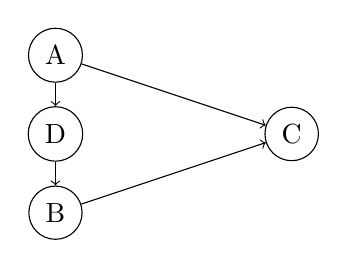
\begin{tikzpicture}
	\node[shape=circle,draw=black] (A) at (0,1) {A};
	\node[shape=circle,draw=black] (B) at (0,-1) {B};
	\node[shape=circle,draw=black] (C) at (3,0) {C};
	\node[shape=circle,draw=black] (D) at (0,0) {D};
	\draw[->] (A) edge (D);
	\draw[->] (D) edge (B);
	\draw[->] (A) edge (C);
	\draw[->] (B) edge (C);
	%\draw[color=gray] (0,0) -. (C);
	\end{tikzpicture}
\end{center}
The optimal flow stays the same
\begin{align*}
f = \begin{pmatrix}
1&0\\0&1\\0&0\\0&0
\end{pmatrix}
\end{align*}
and we get optimal duals $\phi_A = (l,l)$, $\phi_B = (l,l)$, $\phi_C = (0,0)$, $\phi_D = (h,h)$. One can again directly check that all constraints are satisfied. To see if $D\phi$ is feasible, by symmetry it suffices to consider the triangle $DCA$. Here,
\[
D\phi = \begin{pmatrix}
-1&l-h\\-1&l-h
\end{pmatrix}.
\]
Then $\lVert e_i^T D\phi \rVert^2 = \lVert (-1,l-h) \rVert^2 = 1 + (l-h)^2 > 1$, so the dual solution is still not feasible.
\section{Shortest path}
Consider
\begin{center}

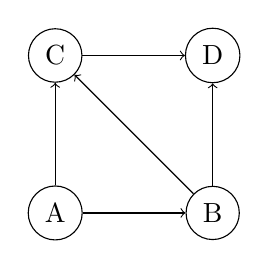
\begin{tikzpicture}[scale = 2]
\node[shape=circle, draw=black] (A) at (0,0) {A};
\node[shape=circle, draw=black] (B) at (1,0) {B};
\node[shape=circle, draw=black] (C) at (0,1) {C};
\node[shape=circle, draw=black] (D) at (1,1) {D};
\draw[->] (A) edge (B)  edge (C);
\draw[->] (B) edge (D);
\draw[->] (C) edge (D);
\draw[->] (B) edge (C);
\end{tikzpicture}
\end{center}
With supply $1$ at $A$ und $-1$ at $D$. An optimal solution is
\begin{align*}
f = \begin{pmatrix}
1\\0\\0\\1\\0
\end{pmatrix}
\end{align*}
(where edges are ordered lexicographically). An optimal dual solution is $\phi_A = 2$, $\phi_B = 1$, $\phi_C = 1$, $\phi_D = 0$. In the triangle $BDC$, $D\phi = (-1 -1)$ which suggests an edge in the $(1,1)$-direction. In the triangle $ABC$, $D\phi = (-1 -1)$ as well. Hence, we refine the traingulation and get
\begin{center}
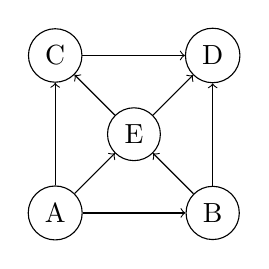
\begin{tikzpicture}[scale = 2]
\node[shape=circle, draw=black] (A) at (0,0) {A};
\node[shape=circle, draw=black] (B) at (1,0) {B};
\node[shape=circle, draw=black] (C) at (0,1) {C};
\node[shape=circle, draw=black] (D) at (1,1) {D};
\node[shape=circle, draw=black] (E) at (0.5,0.5) {E};
\draw[->] (A) edge (B)  edge (C);
\draw[->] (B) edge (D);
\draw[->] (C) edge (D);
\draw[->] (B) edge (E);
\draw[->] (E) edge (C);
\draw[->] (A) edge (E);
\draw[->] (E) edge (D);
\end{tikzpicture}
\end{center}
The optimal flow now is
\[
f_{AE}=f_{ED}=1
\]
with duals $\phi_A = \sqrt{2}$, $\phi_B = 1/\sqrt{2}$, $\phi_C = 1/\sqrt{2}$, $\phi_D = 0$, $\phi_E = 1/\sqrt{2}$. This is obviously the ``correct'' optimal solution. Consider now $D\phi$ on all $4$ triangles. In $ABE$, $D\phi = (-1/\sqrt{2},-1/\sqrt{2})$ which has norm $1$. By symmetry, this also holds for all other triangles. Hence in this example we indeed terminate with the optimal solution after one refinement.
\section{Steiner tree}
Consider
\begin{center}
	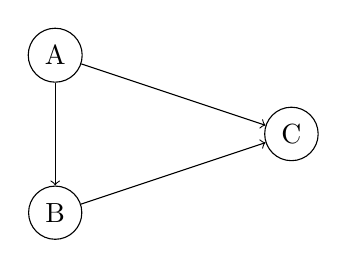
\begin{tikzpicture}
	\node[shape=circle, draw=black] (A) at (0,1) {A};
	\node[shape=circle, draw=black] (B) at (0,-1) {B};
	\node[shape=circle, draw=black] (C) at (3,0) {C};
	\draw[->] (A) edge (C);
	\draw[->] (A) edge (B);
	\draw[->] (B) edge (C);
	\end{tikzpicture}
\end{center}
where the distance from $A$ to $B$ is $1$ and the distance from $AB$ to $C$ is $h=3$, so the distance from $A$ to $C$ is $l = \sqrt{10}$. The supplies are $s_A = (1,0)$, $s_B = (0,1)$ and $s_C = (-1,-1)$. We use the cost function
\[
c(x,y) = \max(x,y,0) + \max(-x,-y,0),
\]
so we consider the Steiner tree problem. An optimal flow is given by $f_{AB} = (1,0)$, $f_{BC} = (1,1)$. Choosing $\phi_C = (0,0)$, $\phi_B$ must lie in $l\partial c(1,1)$, so $\phi_B = (l\lambda,l(1-\lambda))$ for some $\lambda \in [0,1]$. Additionally, $\phi_A-\phi_B \in 2\partial c(1,0)$, so $\phi_A = (l\lambda,l(1-\lambda)) + (2,2\mu)$ for a $\mu \in [-1,1]$. We choose $\mu = -1$ and
\[
\lambda = 0,
\]
so $\phi_B = (0,l)$ and $\phi_A = (2, l-2)$. One can check that $\phi_A \in l\partial c(0,0)$, so we indeed constructed an optimal dual solution. The differential $D\phi$ is given by
\begin{align*}
D\phi = \begin{pmatrix}
-1/h&1\\(1-l)/h&-1
\end{pmatrix}.
\end{align*}
In terms of inequalities, $\partial c(0,0)$ can be written as
\begin{align*}
\partial c(0,0) = \{x: |e_i^T x| \leq 1 \text{ and } |(1,1) x| \leq 1 \}.
\end{align*}
We have $\lVert e_1^T D\phi \rVert^2 = 1 + 1/h^2 = 10/9$, $\lVert e_2^T D\phi \rVert = (1-l)^2/h^2 + 1 \approx 1.5$ and $\rVert (1,1)D\phi \lVert= l^2/h^2 = 10/9$. The largest relative and absolute error comes from $e_2$, and $e_2^T D\phi = ((1-l)/h,-1)$. Note that the angle between an edge in this direction and  $AB$ is approximately $62^\circ$, which is quite close to the correct edge direction.
\end{document}